\chapter{Testy}
\section{Testy w Akka.net}
W Akka.net testy pisze się za pomocą specjalnej pakietu Akka.TestKit wystawiającego zestaw narzędzi do testowania aktorów. Pozwala to na 
przeprowadzenie testów integracyjnych łączących w jednym teście większość stworzonych aktorów. Testy te odzwierciedlają realne sytuacje spotykane w firmach wynajmujących biura. 

Testy najczęściej mają podobną strukturę:
\begin{enumerate}
    \item Stworzenie aktora.
    \item Przesłanie mu wiadomości inicjalizujących (jeżeli jest taka potrzeba.)
    \item Wysłanie wiadomości uruchamiającej testowane zachowane aktora.
    \item Odczytanie zwróconej wiadomości i sprawdzenie czy wartości wewnątrz zgadzają się z oczekiwaniami
\end{enumerate}
Istotne jest zauważenie różnicy w stosunku do testów jednostkowych. Nie sprawdza się stanu wewnętrznego aktora, lecz jego reakcje na wiadomości.

\section{Scenariusze testowe}
Poniższe scenariusze testowe pozwalają sprawdzić na ile system spełnia założenia opisane w sekcji \ref{sec:wymagania}. Każdy ze scenariuszy testowych opisuje sytuację, która może wydarzyć się zwyczajnego dnia w biurze.

\subsection{Nagłe dodanie spotkania}
Ten scenariusz przewiduje dodanie niespodziewanego spotkania (np. spotkania zespołu w związku z raportem od klienta). Taka ingerencja w kalendarz firmowy powoduje, że wcześniej zaplanowane chłodzenie pomieszczenia musi zostać przyspieszone. 

\begin{lstlisting}
    07:30 - w sali do spotkań panuje temperatura 25st.C
    Zaplanowane jest spotkanie na 10:30 kończące się o 12:00 z wymaganą temperaturą 21st.C
    08:30 - dyrektor dodaje spotkanie spotkanie z zespołem na 09:00 kończące się o 10:00 z wymaganą temperaturą 18st.C
    09:00 - w sali powinna panować temperatura 18st.C +- 0.5st.C
    10:00 - w sali powinna panować temperatura 18st.C +- 0.5st.C
    10:30 - w sali powinna panować temperatura 21st.C +- 0.5st.C
    12:00 - w sali powinna panować temperatura 21st.C +- 0.5st.C
    12:10 - wszystkie urządzenia w sali powinny być wyłączone
\end{lstlisting}

Wyniki testu zostały przedstawione na rysunku \ref{fig:AddSuddenMeeting}.
Zatem proponowane rozwiązanie radzi sobie z nagłą potrzebą przyspieszenia pracy urządzeń HVAC. 
\begin{figure}[hb]
    \centering
    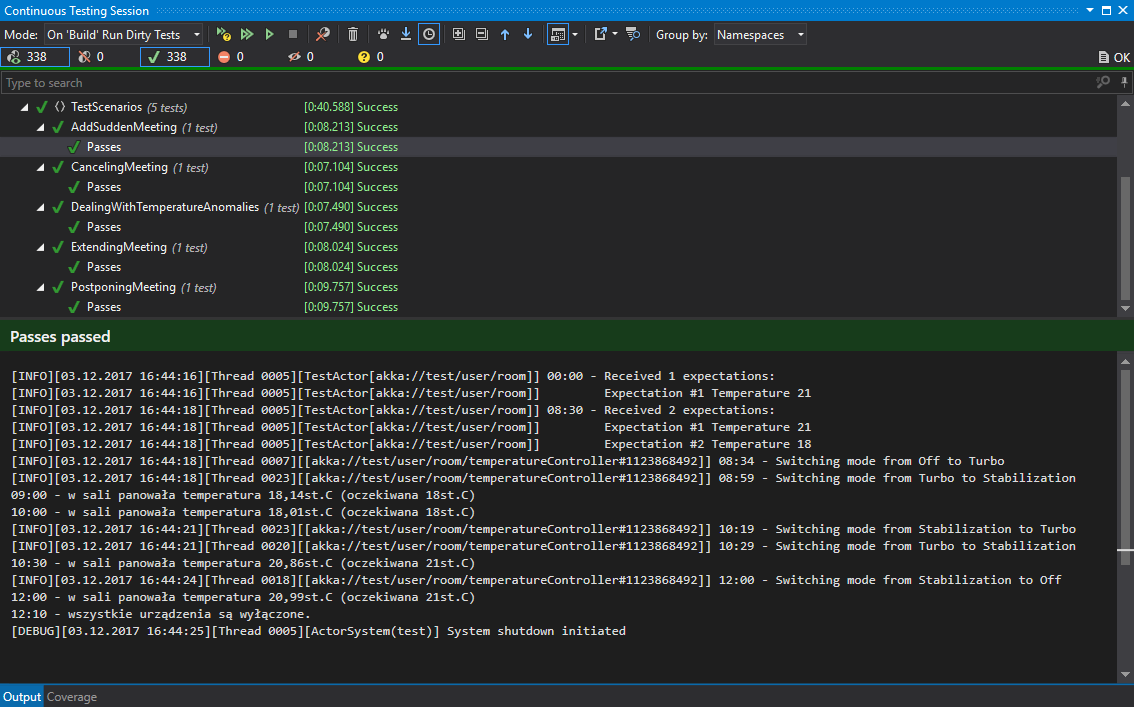
\includegraphics[width=0.90\textwidth]{./screenshots/AddSuddenMeeting.png}
    \caption{Wyniki testu scenatiusza z nagłym dodaniem spotkania}
    \label{fig:AddSuddenMeeting}    
\end{figure}

\subsection{Odwołanie spotkania}
Niejednokrotnie w firmach zdarza się sytuacja, gdy klient lub umówiony współpracownik nie może przybyć na spotkanie i odwołuje je w ostatniej chwili.
Jeżeli system nie barłby tego pod uwagę, koszty pracy urządzeń nie byłyby w pełni optymalizowane. System powinien wyłączać niepotrzebnie pracujące urządzenia.
\begin{lstlisting}
    07:30 - w sali do spotkań panuje temperatura 25st.C
    Zaplanowane są dwa spotkania:
     -spotkanie z klientem na 9:00 kończące się o 10:00 z wymaganą temperaturą 18st.C    
     -spotkanie zespołu na 10:30 kończące się o 12:00 z wymaganą temperaturą 21st.C
    08:30 - do recepcji dzwoni klient i odwołuje spotkanie
    09:00 - wszystkie urządzenia w sali powinny być wyłączone
    10:30 - w sali powinna panować temperatura 21st.C +- 0.5st.C
    12:00 - w sali powinna panować temperatura 21st.C +- 0.5st.C
    12:10 - wszystkie urządzenia w sali powinny być wyłączone
\end{lstlisting}

Wyniki testu zostały przedstawione na rysunku \ref{fig:CancelledMeeting}.
System wyłączył urządzenia po otrzymaniu sygnału o odwołaniu jednego ze spotkań. W ten sposób zaoszczędził dodatkową energię potrzebną wcześniej na przygotowanie sali do pierwszego spotkania. 
\begin{figure}[p]
    \centering
    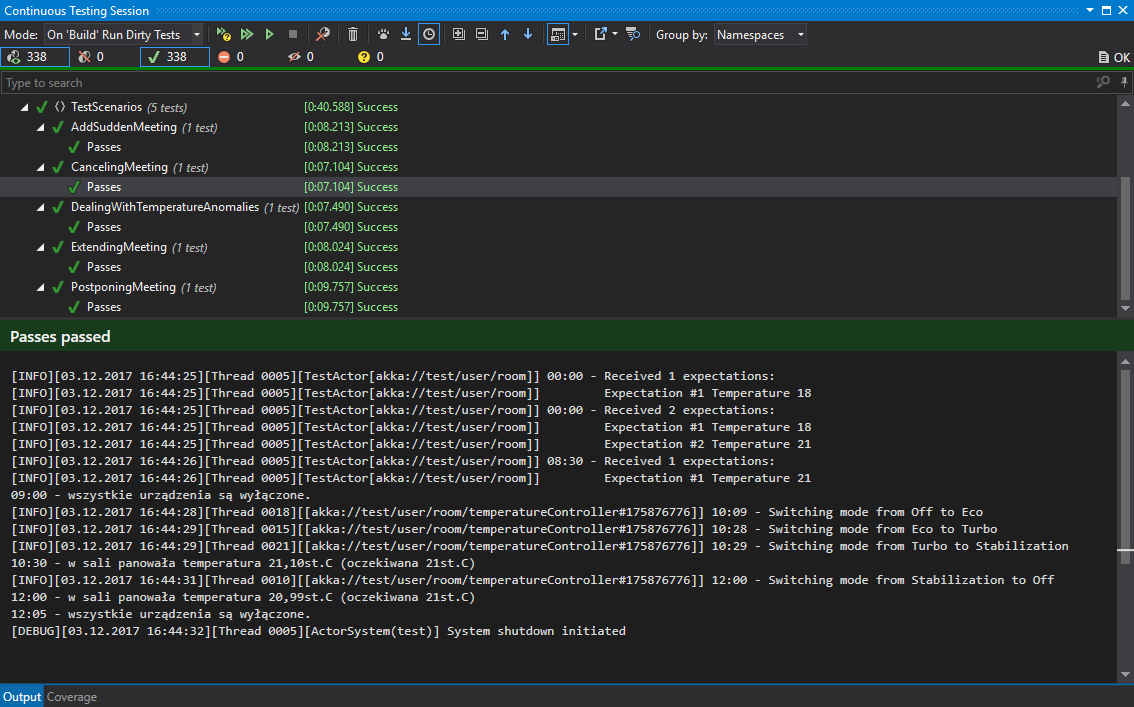
\includegraphics[width=0.90\textwidth]{./screenshots/CancelledMeeting.png}
    \caption{Wyniki testu scenatiusza z odwołanym spotkaniem}
    \label{fig:CancelledMeeting}    
\end{figure}

\subsection{Przesunięcie spotkania}
Czasami zamiast odwoływać spotkanie, klient proponuje przesunięcie go o od kilku minut od kilku godzin. 
System powinien w takiej sytuacji przesunąć dostosowywanie pomieszczenia zgodnie z nową, późniejszą godziną rozpoczęcia spotkania.
\begin{lstlisting}
    07:30 - w sali do spotkań panuje temperatura 25st.C
    Zaplanowane jest spotkanie na 9:00 kończące się o 12:00 z wymaganą temperaturą 18st.C
    08:30 - spotkanie zostaje przesunięte na 11:00 do 14:00
    09:00 - wszystkie urządzenia w sali powinny być wyłączone
    11:00 - w sali powinna panować temperatura 18st.C +- 0.5st.C
    14:00 - w sali powinna panować temperatura 18st.C +- 0.5st.C
    14:05 - wszystkie urządzenia w sali powinny być wyłączone
\end{lstlisting}

Wyniki testu zostały przedstawione na rysunku \ref{fig:PostponedMeeting}.
System wstrzymał pracę urządzeń do momentu, gdy były potrzebne do przygotowania sali do przesuniętego spotkania.
\begin{figure}[p]
    \centering
    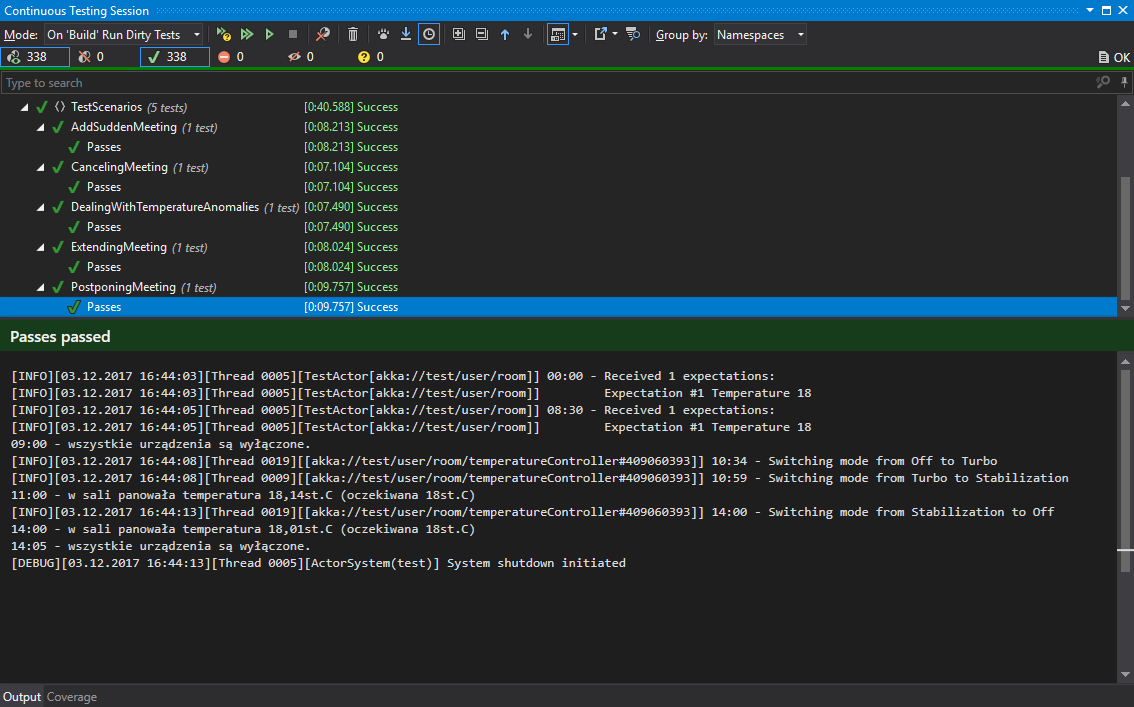
\includegraphics[width=0.90\textwidth]{./screenshots/PostponedMeeting.png}
    \caption{Wyniki testu scenatiusza z przesuniętym spotkaniem}
    \label{fig:PostponedMeeting}    
\end{figure}

\subsection{Przedłużenie spotkania}
Spotkania zespołów produkcyjnych, a zwłaszcza planowanie na początku miesiąca często się przedłuża o kwadrans do pół godziny. System powinien przedłużyć okres klimatyzowania pomieszczenia o czas, który podali użytkownicy.
\begin{lstlisting}
    07:30 - w sali do spotkań panuje temperatura 25st.C
    Zaplanowane jest spotkanie na 9:00 kończące się o 11:00 z wymaganą temperaturą 18st.C
    09:00 - w sali powinna panować temperatura 18st.C +- 0.5st.C
    10:45 - spotkanie zostaje przedłużone do 11:30
    11:00 - w sali powinna panować temperatura 18st.C +- 0.5st.C
    11:30 - w sali powinna panować temperatura 18st.C +- 0.5st.C
    11:35 - wszystkie urządzenia w sali powinny być wyłączone
\end{lstlisting}

Wyniki testu zostały przedstawione na rysunku \ref{fig:ExtendedMeeting}.
System podtrzymał żądaną temperaturę przez dodatkowe pół godziny po czym wyłączył urządzenia, gdy nie były już potrzbne.
\begin{figure}[hb]
    \centering
    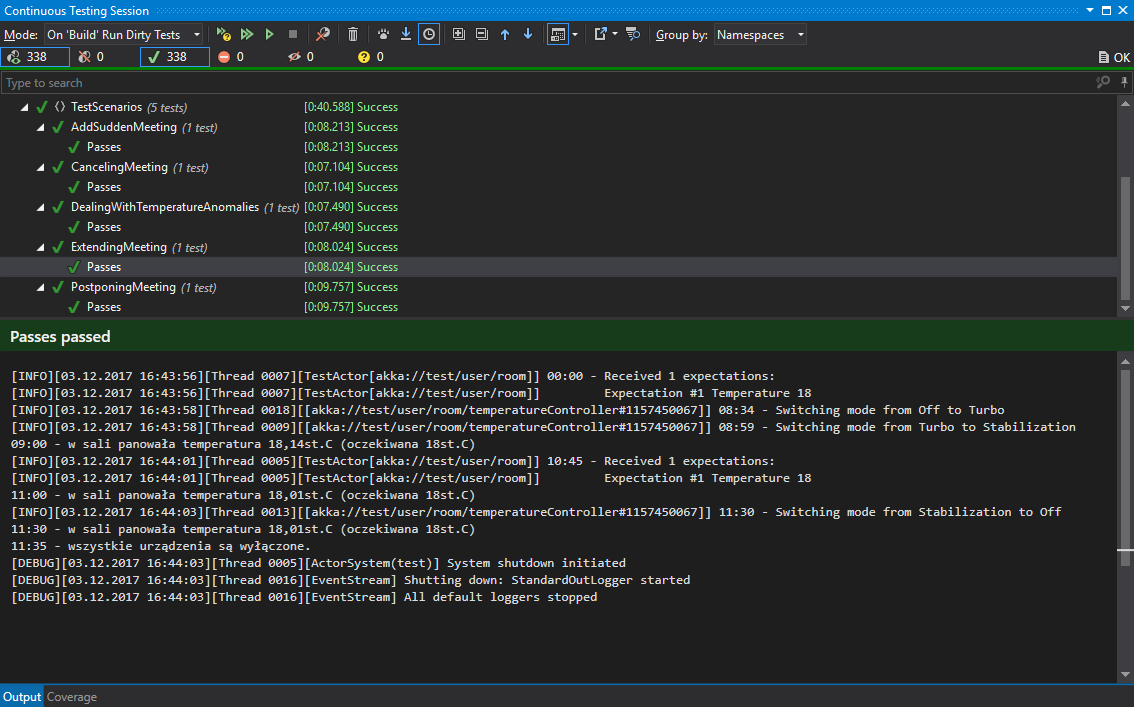
\includegraphics[width=0.90\textwidth]{./screenshots/ExtendedMeeting.png}
    \caption{Wyniki testu scenatiusza z przedłużonym spotkaniem}
    \label{fig:ExtendedMeeting}    
\end{figure}

\subsection{Otwarcie okna - zmiana temperatury niezgodna z modelem}
Czasami mogą nastąpić zmiany temperatury niezgodne z wyliczeniami modelu. 
Przykładem może być uchylenie okna w zimowy dzień. 
System powinien zareagować jeżeli temperatura odbiegnie od tej której zakładał w obliczeniach i dostosować nowy tryb pracy do warunków w pomieszczeniu.
\begin{lstlisting}
    07:30 - w sali do spotkań panuje temperatura 20st.C
    Zaplanowane jest spotkanie na 9:00 kończące się o 11:00 z wymaganą temperaturą 23st.C
    08:30 - otwarcie okna powoduje spadek temperatury do 18st.C 
    09:00 - w sali powinna panować temperatura 23st.C +- 0.5st.C
    11:00 - w sali powinna panować temperatura 23st.C +- 0.5st.C
    11:05 - wszystkie urządzenia w sali powinny być wyłączone
\end{lstlisting}

Wyniki testu zostały przedstawione na rysunku \ref{fig:TemperatureAnomalies}.
System poradził sobie z nagłym spadkiem temperatury, jednak musiał przez to włączyć bardziej kosztowny tryb klimatyzatorów.
\begin{figure}[hb!]
    \centering
    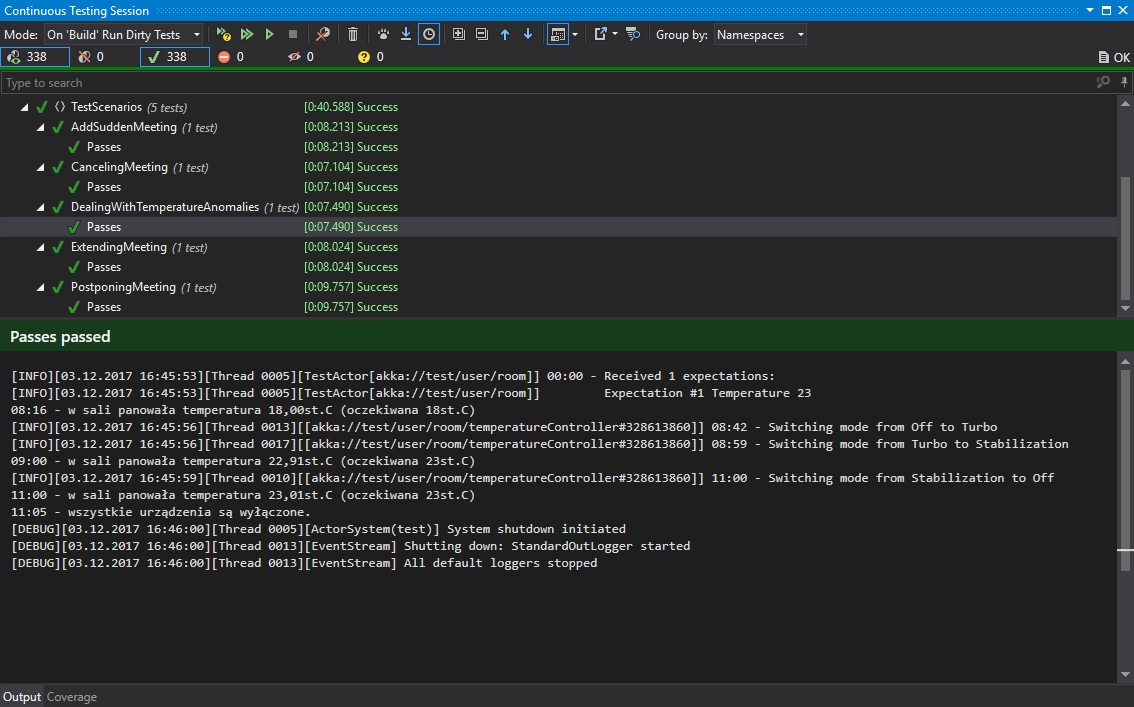
\includegraphics[width=0.90\textwidth]{./screenshots/TemperatureAnomalies.png}
    \caption{Wyniki testu scenatiusza z temperaturą niezgodną z modelem}
    \label{fig:TemperatureAnomalies}    
\end{figure}

\section{Pułapki związane z testowaniem aktorów}
Podczas przeprowadzania testów integracyjnych i jednostkowych zdefiniowano pewne zasady, którymi warto się kierować podczas opracowywania testów w Akka.net.

\subsection{Sprawdzanie stanu wewnętrznego aktora}
Mimo tego, że Akka.TestKit udostępnia metody pozwalające na sprawdzenie stanu wewnętrznego aktora, nie jest to zalecane podejście. 
Prowadzi do sytuacji, gdzie testy zależą od wewnętrznej implementacji. 
Tak jak w tradycyjnych testach jednostkowych testuje się implementacje interfejsów, tak w Akka.net testuje się zachowania na poszczególne obsługiwane wiadomości.

\subsection{Używanie metody \lstinline{Ask} }
\lstinline{Ask<T>} jest metodą pozwalającą oczekiwać na wiadomość zwrotną z systemu aktorów danego typu \lstinline{T}.
Jest ona częścią wewnętrznych mechanizmów Akka.net i sami twórcy nie zalecają jej używania wewnątrz pisanych aktorów \cite{bib:AkkaNoAsk}. 
\lstinline{Ask<T>} nie pozwala na zmianę wątku, co w przypadku testów doprowadza do sytuacji, gdzie test zwraca błąd związany z przekroczeniem czasu oczekiwania na wiadomość zwrotną. Zamiast tego, w testach powinna występować metoda \lstinline{ExpectMsg<T>}, która zwraca pierwszą wiadomość typu \lstinline{T}, która przyjdzie do aktora testowego dostępnego w klasie \lstinline{TestKit}.  